% -----------------------------------------------------------------------------
% ########################
% # PREDLOGA ZA POROCILO #
% ########################
%
% @author Iztok Starc
% @date   3. december 2008
%
\documentclass[a4paper,12pt]{report}

% -----------------------------------------------------------------------------
% ####################################################
% # UPORABA PAKETOV - NASTAVITEV JEZIKA in KODIRANJA #
% ####################################################
\usepackage[slovene]{babel}
\usepackage[utf8]{inputenc}
\usepackage{lmodern}
\usepackage[T1]{fontenc}
\usepackage[sc]{mathpazo}
\linespread{1.05}
\usepackage[T1]{fontenc}

% -----------------------------------------------------------------------------
% ######################################
% # VNOS KLJUCNIH PARAMETROV BESEDILA  #
% ######################################

\newcommand{\naslov}     {EPOS}
\newcommand{\prviavtor}  {David Ocepek}
\newcommand{\prviindeks} {63160248}
\newcommand{\drugiavtor} {Jana Novak}
\newcommand{\drugiindeks}{63000001}
\newcommand{\tretjiavtor} {Marija Novak}
\newcommand{\tretjiindeks}{63000002}
\newcommand{\kraj}       {Ljubljana}

% -----------------------------------------------------------------------------
% ###################
% # UPORABA PAKETOV #
% ###################
\usepackage[a4paper,left=25mm,right=25mm,top=20mm,bottom=30mm,includehead]{geometry}

\usepackage{graphicx, epsfig}

\usepackage{fancyhdr}

\usepackage[
colorlinks=true, linkcolor=blue, citecolor=red,
%
pdftitle={\naslov},
pdfauthor={\prviavtor, \drugiavtor},
pdfsubject={Poročilo seminarske naloge pri predmetu Elektronsko Poslovanje},
pdfkeywords={spletna prodajalna, PHP, SSL, MySQL}, a4paper, pagebackref=true, unicode]{hyperref}

% -----------------------------------------------------------------------------
\begin{document}

% -----------------------------------------------------------------------------
% ##################
% # NASLOVNA STRAN #
% ##################
\begin{titlepage}
	\begin{center}
	{UNIVERZA V LJUBLJANI\\[10pt] 
	FAKULTETA ZA RAČUNALNIŠTVO IN INFORMATIKO}

	\vspace{65mm}

	{\Large\textbf{\naslov}}

	\vspace{10mm}

	{\large Poročilo seminarske naloge pri predmetu\\[10pt] Elektronsko poslovanje}

	\vfill
	\vspace{60mm}

\hspace{20mm}
\begin{minipage}[t]{70mm}
	{\bf Študenti}\\
	{\prviavtor} ({\prviindeks})\\ 
\end{minipage}
%\hfill
\begin{minipage}[t]{50mm}
	{\bf Mentor}\\
	David Jelenc
\end{minipage}
%\hspace{20mm}

	\vspace{35mm}

	{	\kraj, \today}
	\end{center}
\end{titlepage}

% -----------------------------------------------------------------------------
% ##################
% # KAZALO VSEBINE #
% ##################

\tableofcontents

% -----------------------------------------------------------------------------
% ############
% # POVZETEK #
% ############
%\begin{abstract}
%\end{abstract}

% -----------------------------------------------------------------------------
% ##################
% # UVOD DOKUMENTA #
% ##################
\chapter{Uvod}

Tema seminarske naloge je model spletne trgovine implementirana z uporabo Linux, Apache, SUPB MySQL, PHP, SSL, certifikatov X.509 in mobilne platforme Android.

% -----------------------------------------------------------------------------
% ###################
% # JEDRO DOKUMENTA #
% ###################

% -----------------------------------------------
\chapter{Navedba realiziranih storitev}

\section{Osnovne storitve}

Implementirane so vse osnovne storitve.

\section{Razširjene storitve}

Spletna prodajalna je smiselno organizirano s pomočjo tehnologij CSS in JavaScript. Zgrajena je po vzorcu MVC in vsi klici na Controller uporabljajo AJAX.


% -----------------------------------------------
\chapter{Podatkovni model}

\begin{figure}[htb]
	\centering
	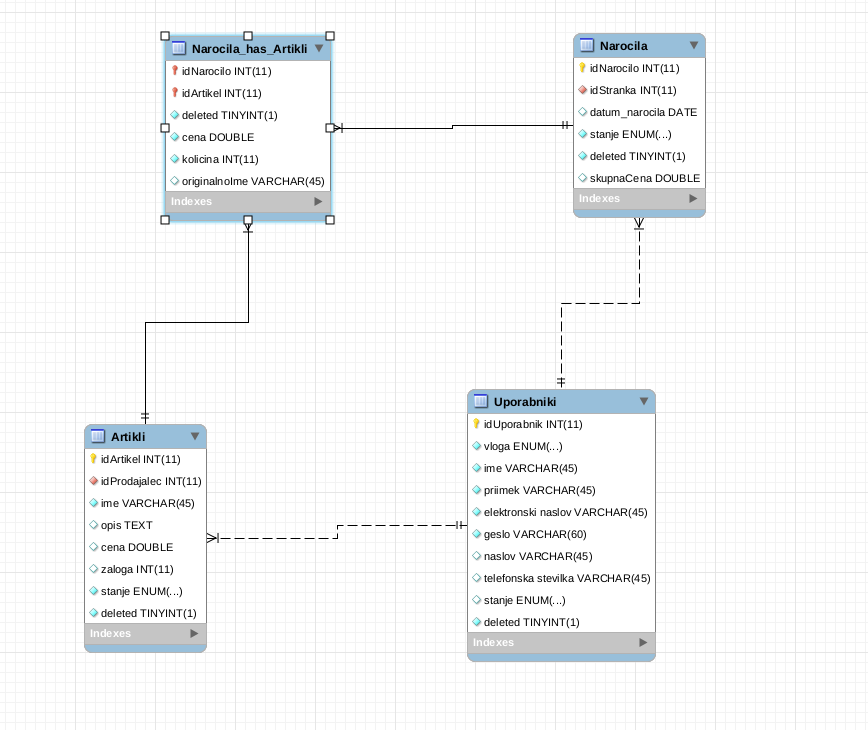
\includegraphics[width=13cm]{img/baza.png}
	\caption{Slika določenega vzorca}
\label{fig:1}
\end{figure}

\section{Uporabniki}

Tabela Uporabniki vasebuje vse podatke o uporabniku, uporabljana je pri vseh vlogah (tj. administrator, prodajalec, stranka).
V primeru da vloga ni stranka sta atributa telefonska stevilka in naslov enaka null.

\section{Artikli}

Tabela Artikli vsebuje vse podatke o artiklu, njegovo ime, opis in ceno ter stanje (tj. ali je aktiviran ali deaktiviran).

\section{Narocila}

Tabela narocila vsebuje podatke o narocilu, idNarocila, idStranke, kateri narocilo pripada, stanje narocila in skupnoCeno narocila, ki je agregirana vrednost vsih artiklov v narocilu in je prisotna, ker jo je pogosto traba racunati in povecuje potrebo po posiljanju dodatnih requestov bazi in Controllerju.

\section{Narocila\_has\_Artikli}

Tabela vsebuje seznam artiklov v narocilu kot par (idNarocilo, idArtikel). Vsebuje takratno ceno artila, takratno ime artikla in stevilo kupljenih artiklov kot kolicino. 



% -----------------------------------------------
\chapter{Varnost sistema}

\begin{center}
\resizebox{\textwidth}{!}{\begin{tabular}{ |c|c|c| } 
 \hline
 Mehanizem & razlog \\ 
 uporaba PDO za vse poizvedbe & preprečevanje SQL vstavljanja \\
uporaba htmlspecialchar za vse vnose & preprečevanje XSS vstavljanja v HTML \\ 
Controller output kodiran v JSON & preprečevanje XSS vstavljanja v PHP \\
Neuporaba neznanih spremenljivk kot imput javascript funkcijam & preprečevanje XSS vstavljanja v JS \\ 
Shranjevanje dovoljen v seji & preprečevanje sreminjanja dovoljenj \\ 
Regeneriranje id seje & preprečevanje tujih sej \\ 
Preverjanje dovoljenj pri vsemi akcijah & preprečevanje navtoriziranih akcij \\
Uporaba SSL certifikata & omojevanje uporabe tujih uporabniskih racunov \\
HTTPS enkripcija & kriptiranje podatkov pred nezazeljenimi gledalci \\
 \hline
\end{tabular}}
\end{center}

% -----------------------------------------------
\chapter{Izjava o avtorstvu seminarske naloge}

Spodaj podpisani \textit{\prviavtor}, vpisna številka \textit{\prviindeks}, sem (avtor seminarske naloge z naslovom \textit{\naslov}. S svojim podpisom zagotavljam, da sem izdelal seminarsko nalogo sam.

Podpis: {\prviavtor}, l.r. 

\newpage

% -----------------------------------------------------------------------------
% #######################
% # ZAKLJUCEK DOKUMENTA #
% #######################
\chapter{Zaključek}

Aplikacija EPOS vsebuje vse dele modernih spletnih aplikacij ter enostaven Android vmesnik.


% -----------------------------------------------------------------------------
% ##############
% # LITERATURA #
% ##############
\begin{thebibliography}{99}
\addtocounter{chapter}{1}
\addcontentsline{toc}{chapter}{\protect\numberline{\thechapter}Literatura}
\addtocontents{toc}{\protect\vspace{15pt}}

\bibitem{bib:IPsecHowTo1} Denis Trček; Devid Jelenc \emph{Elektronsko poslovanje} (online). 2003. (citirano \today). Dostopno na naslovu:
\url{https://ucilnica.fri.uni-lj.si/course/view.php?id=113}

\end{thebibliography}

\end{document}
